\documentclass{article}
\usepackage[utf8]{inputenc}
\usepackage{amsmath,amssymb}
\usepackage{graphicx}
\usepackage{booktabs}
\usepackage{hyperref}
\usepackage{natbib}
\usepackage{xcolor}
\usepackage{multirow}
\usepackage{tikz}
\usetikzlibrary{arrows.meta,positioning,shapes.geometric,fit,backgrounds,calc}

% Preprint margins
\usepackage[margin=1in]{geometry}

\title{Self-Supervised Discovery of Discrete Network States\\in Brain Organoid Recordings}

\author{
  Ishara R. Pathirana\\
  Independent Researcher\\
  \texttt{iiaishara@gmail.com}
}

\date{}

\begin{document}

\maketitle

% ============================================================
% ABSTRACT
% ============================================================
\begin{abstract}
Brain organoids cultured on multi-electrode arrays (MEAs) generate complex spontaneous activity, but characterizing their network dynamics typically requires hand-designed features and supervised classification. We introduce SOMA (Self-Organized MEA Architecture), a self-supervised Vision Transformer trained via Joint Embedding Predictive Architecture (JEPA) on spike-binned MEA recordings, that discovers discrete network states without any labels or prior assumptions. Applied to 4.9 days of continuous recording from a human brain organoid (32 electrodes, 2.6M spike events), SOMA identifies a hierarchical state structure: 4 coarse states at 128-dim embedding (silhouette$=0.325$) resolving to 9 fine-grained states at 256-dim (silhouette$=0.636$). The coarse structure---a bistable baseline punctuated by transient bursts---is validated by split-half reliability: four independently trained models on non-overlapping data discover identical state structure with $<1\%$ proportion difference and silhouette scores up to 0.703. The learned representations also capture a developmental trajectory: state entropy increases from 0.51 to 1.92 bits over 5 recording days, consistent with neural network maturation. To our knowledge, this is the first application of self-supervised transformers to organoid electrophysiology and the first unsupervised discovery of hierarchical network states in brain organoids.
\end{abstract}

% ============================================================
% 1. INTRODUCTION
% ============================================================
\section{Introduction}

Human brain organoids---three-dimensional neural cultures derived from induced pluripotent stem cells---have emerged as promising \textit{in vitro} models for studying human neural development and disease \citep{lancaster2013cerebral, pasca2019assembloids}. When cultured on multi-electrode arrays (MEAs), organoids exhibit spontaneous electrophysiological activity including synchronous bursting, oscillatory patterns, and activity that evolves over developmental timescales \citep{trujillo2019complex, sharf2022functional}. The FinalSpark Neuroplatform provides continuous, long-duration MEA recordings from human brain organoids, enabling longitudinal analysis of network dynamics \citep{jordan2024open}.

Despite the richness of these recordings, analysis of organoid electrophysiology remains largely dependent on hand-crafted features: spike rates, burst detection thresholds, synchrony indices, and other metrics chosen \textit{a priori} by the experimenter. This creates a fundamental limitation: the features assume what patterns are relevant before the data has been examined. Complex, multi-dimensional network states that do not align with predefined features may go undetected entirely.

Self-supervised learning (SSL) offers a principled alternative. Rather than requiring labeled examples of the states we wish to find, SSL trains a model to predict its own internal representations, learning a compressed description of the data's structure. The resulting embedding space can then be interrogated for clusters, trajectories, and other patterns---without any assumptions about what those patterns should look like. SSL methods have shown remarkable success in vision \citep{assran2023ijepa}, language, and, more recently, neural signal analysis \citep{kostas2021bendr, dong2024brainjepa}.

In this work, we introduce SOMA (Self-Organized MEA Architecture), a self-supervised Vision Transformer adapted for spike-binned MEA data (Figure~\ref{fig:architecture}). SOMA uses a Joint Embedding Predictive Architecture (JEPA) with Barlow Twins regularization to learn representations of organoid activity without supervision. Our contributions are:

\begin{enumerate}
    \item We demonstrate that SSL discovers \textbf{discrete, biologically meaningful network states} in organoid MEA recordings---a bistable baseline punctuated by transient bursts---without any labels or feature engineering.
    \item We show these states are \textbf{hierarchically organized}: coarse structure (4 states) at lower model capacity resolves to fine-grained sub-states (9 states) at higher capacity, with monotonically increasing cluster quality.
    \item We validate that discovered states are \textbf{intrinsic to the organoid}: four independently trained models on non-overlapping data recover identical structure with $<1\%$ proportion difference.
    \item We show that the learned representations capture a \textbf{developmental trajectory}: state entropy increases monotonically over 5 recording days, consistent with neural maturation.
\end{enumerate}

To our knowledge, this is the first application of self-supervised transformers to organoid electrophysiology, the first unsupervised discovery of network states in brain organoids, and the first demonstration of hierarchical neural state structure emerging from SSL on MEA data.

% ============================================================
% 2. RELATED WORK
% ============================================================
\section{Related Work}

\paragraph{Organoid electrophysiology.}
\citet{trujillo2019complex} first demonstrated oscillatory activity in human brain organoids recorded via MEA, showing developmental trajectories over months of culture. \citet{sharf2022functional} characterized network dynamics across thousands of electrodes using high-density MEAs, revealing structured spatial patterns. The FinalSpark Neuroplatform \citep{jordan2024open} provides open-access, continuous MEA recordings from human brain organoids, enabling the kind of long-duration analysis we perform here. However, all prior analyses of organoid MEA data have relied on supervised or hand-crafted feature approaches.

\paragraph{Neural state discovery.}
Hidden Markov Models (HMMs) have been applied to cortical culture data to identify discrete network states \citep{beggs2003neuronal}, and similar approaches exist for \textit{in vivo} neural recordings. These methods require explicit state models and assumptions about state dynamics. More recently, variational autoencoders and other generative models have been applied to neural population data, but not to organoid MEA recordings.

\paragraph{Self-supervised learning for neural signals.}
BENDR \citep{kostas2021bendr} applied contrastive self-supervised learning to scalp EEG, demonstrating that SSL representations outperform hand-crafted features for downstream classification. \citet{dong2024brainjepa} introduced Brain-JEPA for fMRI, using JEPA training on BOLD signals at NeurIPS 2024. NeuroGPT \citep{cui2024neurogpt} applied masked prediction pretraining to scalp EEG. Critically, none of these works address MEA recordings or brain organoids---our work fills this gap.

\paragraph{JEPA architectures.}
The Joint Embedding Predictive Architecture (JEPA) family \citep{assran2023ijepa, bardes2024vjepa} learns representations by predicting target embeddings from context, avoiding pixel-level reconstruction. We adapt this framework to 2D spike matrices (channels $\times$ time bins), treating MEA recordings as ``images'' of neural activity.

% ============================================================
% 3. METHODS
% ============================================================
\section{Methods}

\subsection{Data}

We use recordings from the FinalSpark Neuroplatform \citep{jordan2024open}: a human brain organoid cultured on a 4$\times$8 multi-electrode array (32 electrodes, 30\,kHz sampling rate). The recording spans 4.9 days of continuous monitoring (sample identifier: fs437), yielding 2,636,726 detected spike events across all electrodes. Data includes spike timestamps, amplitudes, and electrode indices.

\subsection{Preprocessing}

Spike events are binned at 100\,ms temporal resolution into $C \times T$ activity matrices, where $C = 32$ (electrodes) and $T = 10$ (time bins per 1-second window). Each element counts the number of spikes detected on electrode $c$ during time bin $t$. Windows are extracted with 1\,s duration and 0.5\,s stride, sampled uniformly across the full recording to ensure all 5 recording days are represented. We use up to 24,740 windows for GPU training and 9,830 for CPU experiments.

Spike counts are log-transformed ($\log(1 + x)$) and standardized per electrode to zero mean and unit variance across the training set.

\subsection{Architecture: SOMA}

SOMA is a self-supervised Vision Transformer adapted for MEA data. The architecture consists of:

\paragraph{Input representation.} Each $32 \times 10$ activity matrix is divided into non-overlapping patches of size $1 \times 10$ (one electrode $\times$ all time bins), yielding 32 patch tokens. Each patch is linearly projected to the embedding dimension $d$ and combined with learned positional embeddings.

\paragraph{JEPA training.} Following \citet{assran2023ijepa}, we use a dual-encoder architecture:
\begin{itemize}
    \item A \textbf{context encoder} $f_\theta$ processes a masked subset of patches (75\% masking ratio).
    \item A \textbf{target encoder} $f_{\bar{\theta}}$ processes all patches without masking. Its weights are an exponential moving average (EMA) of the context encoder: $\bar{\theta} \leftarrow \alpha\bar{\theta} + (1-\alpha)\theta$, with $\alpha = 0.996$.
    \item A \textbf{predictor} $g_\phi$ maps context encoder outputs to predicted target representations.
\end{itemize}

\begin{figure*}[t]
\centering
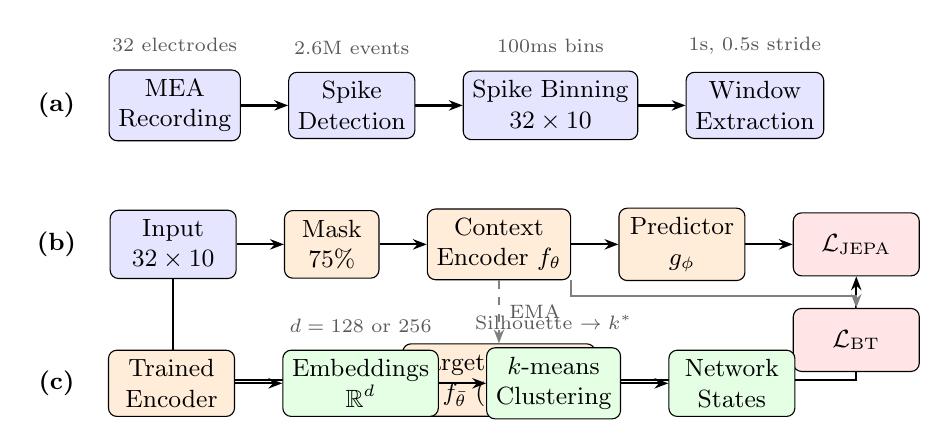
\begin{tikzpicture}[
    node distance=0.6cm and 0.8cm,
    box/.style={draw, rounded corners=3pt, minimum height=0.8cm, minimum width=1.6cm, align=center, font=\small},
    data/.style={box, fill=blue!10},
    model/.style={box, fill=orange!15},
    loss/.style={box, fill=red!10},
    result/.style={box, fill=green!10},
    arrow/.style={-{Stealth[length=5pt]}, thick},
    label/.style={font=\scriptsize, text=gray!70!black},
]

% (a) Data pipeline
\node[font=\small\bfseries] (a_label) {(a)};
\node[data, right=0.3cm of a_label] (mea) {MEA\\Recording};
\node[data, right=0.6cm of mea] (spikes) {Spike\\Detection};
\node[data, right=0.6cm of spikes] (bins) {Spike Binning\\$32 \times 10$};
\node[data, right=0.6cm of bins] (windows) {Window\\Extraction};

\draw[arrow] (mea) -- (spikes);
\draw[arrow] (spikes) -- (bins);
\draw[arrow] (bins) -- (windows);

\node[label, above=0.1cm of mea] {32 electrodes};
\node[label, above=0.1cm of spikes] {2.6M events};
\node[label, above=0.1cm of bins] {100ms bins};
\node[label, above=0.1cm of windows] {1s, 0.5s stride};

% (b) Architecture
\node[font=\small\bfseries, below=1.2cm of a_label] (b_label) {(b)};

\node[data, right=0.3cm of b_label] (input) {Input\\$32 \times 10$};
\node[model, right=0.6cm of input, minimum width=1.2cm] (mask) {Mask\\75\%};
\node[model, right=0.6cm of mask] (ctx_enc) {Context\\Encoder $f_\theta$};
\node[model, right=0.6cm of ctx_enc] (pred) {Predictor\\$g_\phi$};
\node[loss, right=0.6cm of pred] (jepa_loss) {$\mathcal{L}_{\text{JEPA}}$};

% Target branch
\node[model, below=0.8cm of ctx_enc] (tgt_enc) {Target Encoder\\$f_{\bar{\theta}}$ (EMA)};

\draw[arrow] (input) -- (mask);
\draw[arrow] (mask) -- (ctx_enc);
\draw[arrow] (ctx_enc) -- (pred);
\draw[arrow] (pred) -- (jepa_loss);
\draw[arrow] (input) |- (tgt_enc);
\draw[arrow] (tgt_enc) -| (jepa_loss);

% EMA arrow
\draw[arrow, dashed, gray] (ctx_enc) -- node[right, label] {EMA} (tgt_enc);

% Barlow Twins
\node[loss, below=0.4cm of jepa_loss] (bt_loss) {$\mathcal{L}_{\text{BT}}$};
\draw[arrow, gray] (ctx_enc.south east) -- ++(0,-0.2) -| (bt_loss);

% (c) Downstream
\node[font=\small\bfseries, below=1.2cm of b_label] (c_label) {(c)};
\node[model, right=0.3cm of c_label] (embed) {Trained\\Encoder};
\node[result, right=0.6cm of embed] (embeddings) {Embeddings\\$\mathbb{R}^d$};
\node[result, right=0.6cm of embeddings] (cluster) {$k$-means\\Clustering};
\node[result, right=0.6cm of cluster] (states) {Network\\States};

\draw[arrow] (embed) -- (embeddings);
\draw[arrow] (embeddings) -- (cluster);
\draw[arrow] (cluster) -- (states);

\node[label, above=0.1cm of embeddings] {$d = 128$ or $256$};
\node[label, above=0.1cm of cluster] {Silhouette $\to k^*$};

\end{tikzpicture}
\caption{\textbf{SOMA architecture and pipeline.} (a)~MEA spike data is binned into $32 \times 10$ activity matrices. (b)~JEPA training: masked input is processed by the context encoder; unmasked input by an EMA target encoder. The predictor maps context to target space, trained with MSE loss ($\mathcal{L}_{\text{JEPA}}$) plus Barlow Twins regularization ($\mathcal{L}_{\text{BT}}$). (c)~After training, embeddings are clustered via $k$-means with silhouette-based model selection.}
\label{fig:architecture}
\end{figure*}

The training objective minimizes the mean squared error between predicted and target embeddings:
\begin{equation}
    \mathcal{L}_{\text{JEPA}} = \frac{1}{|M|} \sum_{i \in M} \| g_\phi(f_\theta(\mathbf{x}_{\setminus M}))_i - f_{\bar{\theta}}(\mathbf{x})_i \|^2
\end{equation}
where $M$ is the set of masked patch indices.

\paragraph{Barlow Twins regularization.} To prevent representational collapse, we add a Barlow Twins loss \citep{zbontar2021barlow} that encourages the cross-correlation matrix of embedding dimensions (computed over the batch) to approximate the identity:
\begin{equation}
    \mathcal{L}_{\text{BT}} = \sum_i (1 - C_{ii})^2 + \lambda \sum_i \sum_{j \neq i} C_{ij}^2
\end{equation}
where $C$ is the cross-correlation matrix and $\lambda$ is a redundancy reduction weight. The total loss is $\mathcal{L} = \mathcal{L}_{\text{JEPA}} + \beta \mathcal{L}_{\text{BT}}$.

\paragraph{Model configurations.} We train two configurations:
\begin{itemize}
    \item \textbf{CPU:} $d = 128$, 4 transformer layers, $\sim$600K parameters, 25 epochs, 9,830 windows.
    \item \textbf{GPU:} $d = 256$, 6 transformer layers, 5.6M parameters, 50 epochs, 24,740 windows.
\end{itemize}

Both use the AdamW optimizer with learning rate $3 \times 10^{-4}$, batch size 64 (CPU) or 16 (GPU), and cosine learning rate scheduling.

\subsection{State Discovery}

After training, we extract embeddings by passing all windows through the context encoder (without masking). The mean over patch tokens yields a single $d$-dimensional embedding per window.

We apply $k$-means clustering for $k \in \{2, 3, \ldots, 11\}$ and select the optimal $k$ by silhouette score \citep{rousseeuw1987silhouettes}. State characterization includes: spike rate profiles, electrode dominance patterns, transition matrices (within-day), run-length distributions, and per-day state entropy $H = -\sum_s p_s \log_2 p_s$.

\subsection{Split-Half Validation}

To validate that discovered states are intrinsic to the organoid rather than artifacts of a specific training run, we employ split-half reliability with an interleaved design. The full recording is divided into 119 one-hour blocks, alternating assignment to Half~A (even blocks) and Half~B (odd blocks). This interleaving ensures both halves sample all recording days equally, controlling for developmental non-stationarity.

Independent SOMA models are trained from scratch on each half. We compare: (1) optimal $k$, (2) silhouette scores, (3) dominant state proportions, and (4) silhouette curve shape across $k$ values. We performed split-half validation at two scales: CPU (128-dim, 20 epochs, $\sim$2,500 windows per half) and GPU (128-dim, 30 epochs, $\sim$9,000 windows per half).

% ============================================================
% 4. RESULTS
% ============================================================
\section{Results}

\subsection{SOMA Discovers Discrete Network States}

At the CPU scale (128-dim, 4 layers), $k$-means clustering on SOMA embeddings reveals 4 discrete network states with silhouette score 0.325 (Table~\ref{tab:states_cpu}). The states fall into two functional categories: two persistent baseline states (S1, S2) comprising 96.3\% of windows, and two transient burst states (S0, S3) comprising 3.7\%.

\begin{table}[h]
\centering
\caption{Network states discovered by SOMA (CPU, 128-dim, $k=4$).}
\label{tab:states_cpu}
\begin{tabular}{@{}lcccc@{}}
\toprule
State & Proportion & Spike Rate (sp/s) & Dominant Channel & Character \\
\midrule
S0 & 2.8\% & 71.3 & Distributed & Minor burst \\
S1 & 48.3\% & 13.1 & Ch.~23 & Baseline-A \\
S2 & 48.0\% & 6.2 & Ch.~15 & Baseline-B \\
S3 & 1.0\% & 79.8 & Distributed & Major burst \\
\bottomrule
\end{tabular}
\end{table}

The baseline states differ in both overall activity level (13.1 vs.\ 6.2~sp/s) and spatial pattern: S1 is dominated by electrode 23 while S2 is dominated by electrode 15, indicating distinct network configurations rather than simple amplitude scaling.

At the GPU scale (256-dim, 6 layers), the model resolves 9 states with silhouette 0.636---substantially higher than the 4-state CPU model (Figure~\ref{fig:states}). The silhouette score increases monotonically from $k=2$ (0.399) through $k=9$ (0.636), suggesting hierarchical sub-state structure within the coarser groupings.

\begin{figure}[t]
\centering
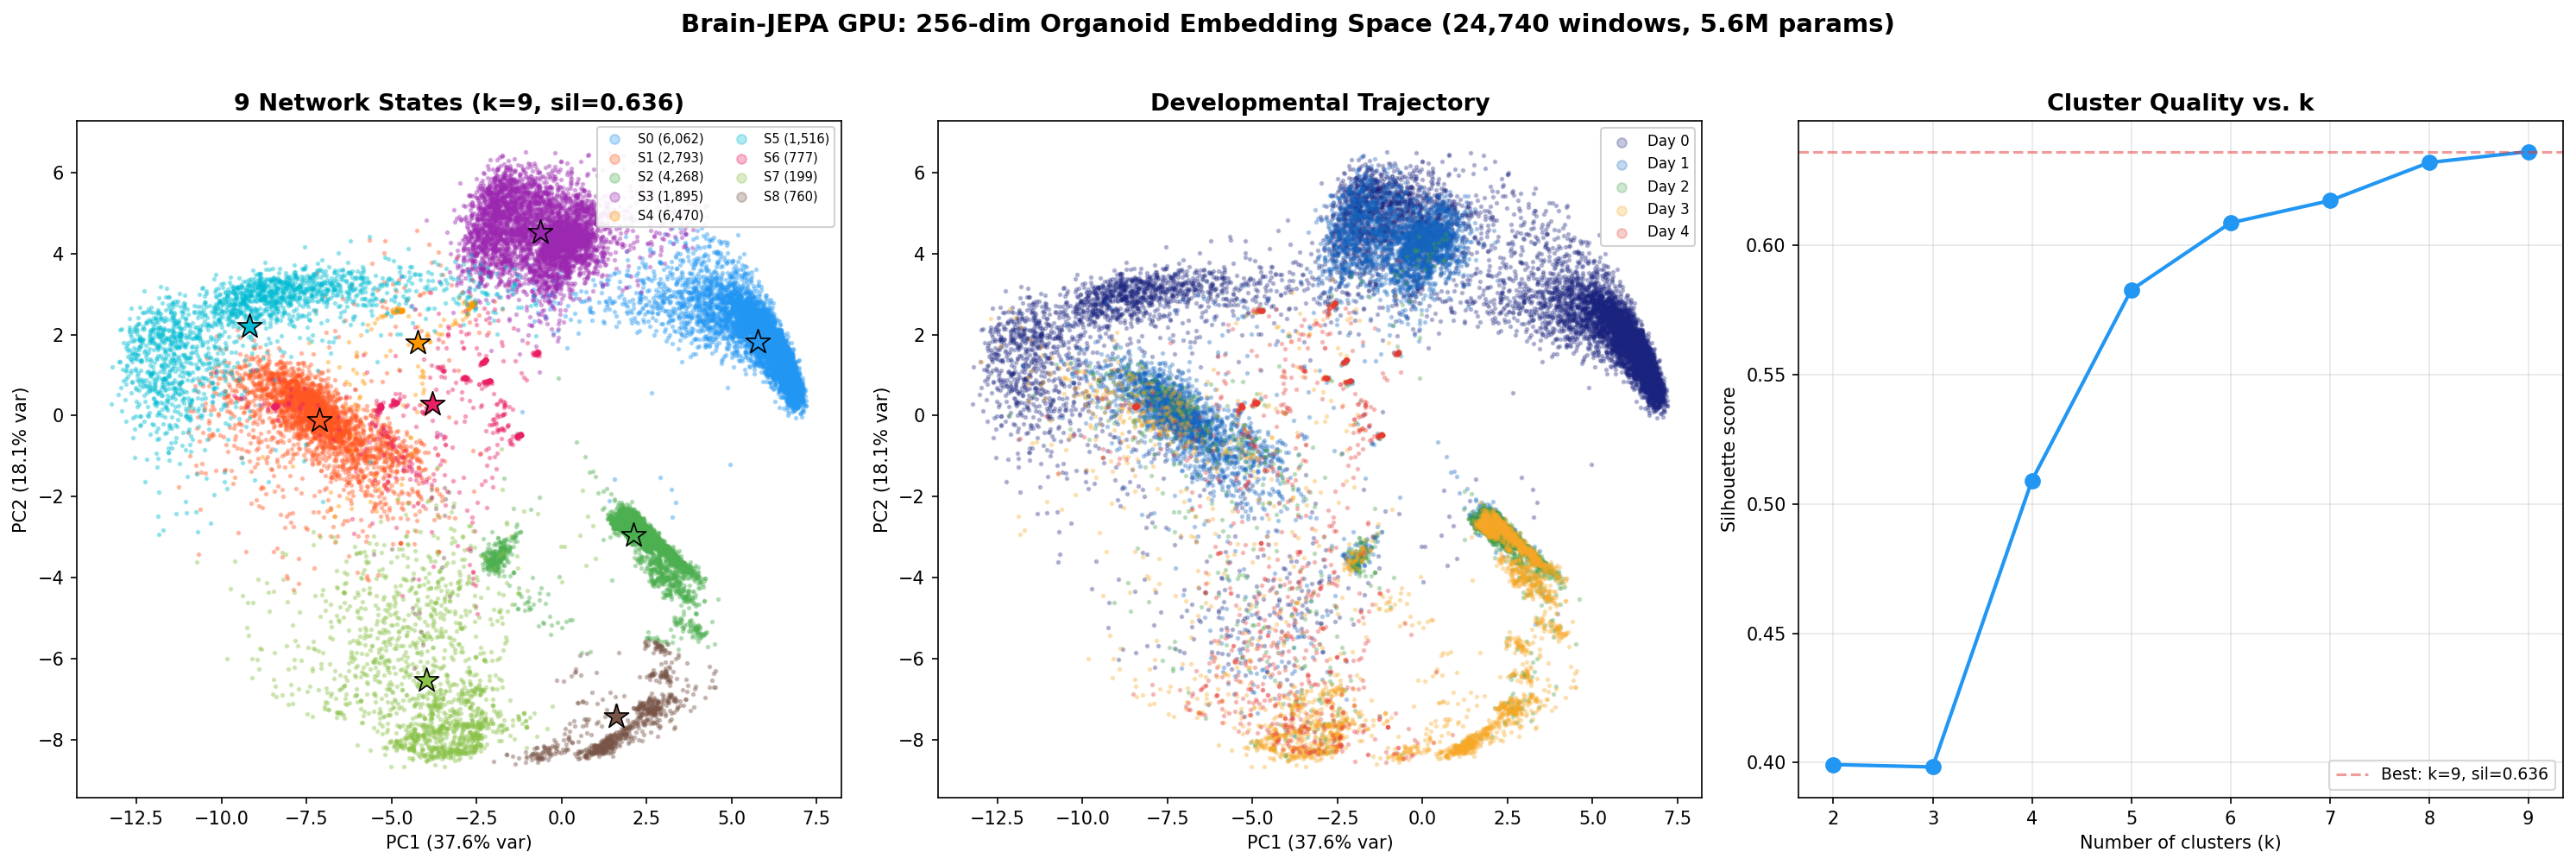
\includegraphics[width=\textwidth]{figures/embedding_visualization.png}
\caption{\textbf{Network states discovered by SOMA (GPU, 256-dim).} Left: PCA projection of 24,740 embeddings colored by 9-state cluster assignment, with centroids marked. Center: Developmental trajectory---embeddings colored by recording day show drift through representation space. Right: Silhouette score as a function of $k$, showing monotonic increase through $k=9$.}
\label{fig:states}
\end{figure}

\subsection{Hierarchical State Organization Across Model Scales}

The same organoid data yields consistent structure across model scales, supporting a hierarchical interpretation (Table~\ref{tab:hierarchy}).

\begin{table}[h]
\centering
\caption{Cross-model robustness: state discovery across SOMA configurations.}
\label{tab:hierarchy}
\begin{tabular}{@{}lccccc@{}}
\toprule
Configuration & Parameters & Windows & $k$ & Silhouette & Interpretation \\
\midrule
128-dim, 4L, 20ep (split-half) & $\sim$600K & $\sim$2,500 & 2 & 0.575--0.625 & Primary binary split \\
128-dim, 4L, 30ep (split-half GPU) & $\sim$600K & $\sim$8,950 & 2 & 0.699--0.703 & Binary split, stronger \\
128-dim, 4L, 25ep & $\sim$600K & 9,830 & 4 & 0.325 & 2 baselines + 2 bursts \\
256-dim, 6L, 50ep & 5.6M & 24,740 & 9 & 0.636 & Sub-states within groups \\
\bottomrule
\end{tabular}
\end{table}

The hierarchy $2 \rightarrow 4 \rightarrow 9$ across increasing model capacity mirrors known properties of neural state spaces. The most fundamental structure---a binary split between two baseline configurations---emerges first with minimal training. Additional model capacity and data reveal finer sub-structure: the two burst modes at $k=4$, then sub-types within each baseline and burst category at $k=9$.

The participation ratio of the 256-dim embedding space is 9.47, confirming that the effective dimensionality matches the number of discovered states. This is not an artifact of over-fitting to noise; the model uses exactly as many dimensions as there are meaningful distinctions in the data.

\subsection{Temporal Dynamics: Persistent Baselines, Transient Bursts}

The discovered states exhibit characteristic temporal dynamics captured by the within-day transition matrix (Table~\ref{tab:transitions}).

\begin{table}[h]
\centering
\caption{State transition probabilities $P(\text{to} \mid \text{from})$, within-day (CPU 4-state model).}
\label{tab:transitions}
\begin{tabular}{@{}lcccc@{}}
\toprule
& $\rightarrow$ S0 & $\rightarrow$ S1 & $\rightarrow$ S2 & $\rightarrow$ S3 \\
\midrule
S0 & 0.390 & 0.184 & 0.327 & 0.099 \\
S1 & 0.009 & \textbf{0.778} & 0.208 & 0.004 \\
S2 & 0.019 & 0.208 & \textbf{0.765} & 0.008 \\
S3 & 0.323 & 0.229 & 0.333 & 0.115 \\
\bottomrule
\end{tabular}
\end{table}

Three key dynamics emerge:

\textbf{Baseline persistence.} States S1 and S2 are highly self-sustaining ($P_{\text{self}} \approx 0.77$) with mean run lengths of 4.5 and 4.3 windows (2.2\,s), respectively.

\textbf{Burst transience.} States S0 and S3 are brief excursions. S3 (major burst) has mean run length 1.1 windows (0.55\,s) and almost never follows itself ($P_{\text{self}} = 0.115$). Both burst states exit preferentially to S2 (low-activity baseline).

\textbf{Baseline bistability.} The S1$\leftrightarrow$S2 transition probability is symmetric ($P \approx 0.208$ in both directions), indicating a balanced bistable system. The organoid spontaneously switches between two stable network configurations, punctuated by rare high-activity bursts.

This dynamical signature---persistent alternation between metastable states with transient burst interruptions---is consistent with reported dynamics in cortical cultures and neural network models near criticality (Figure~\ref{fig:transitions}).

\begin{figure}[t]
\centering
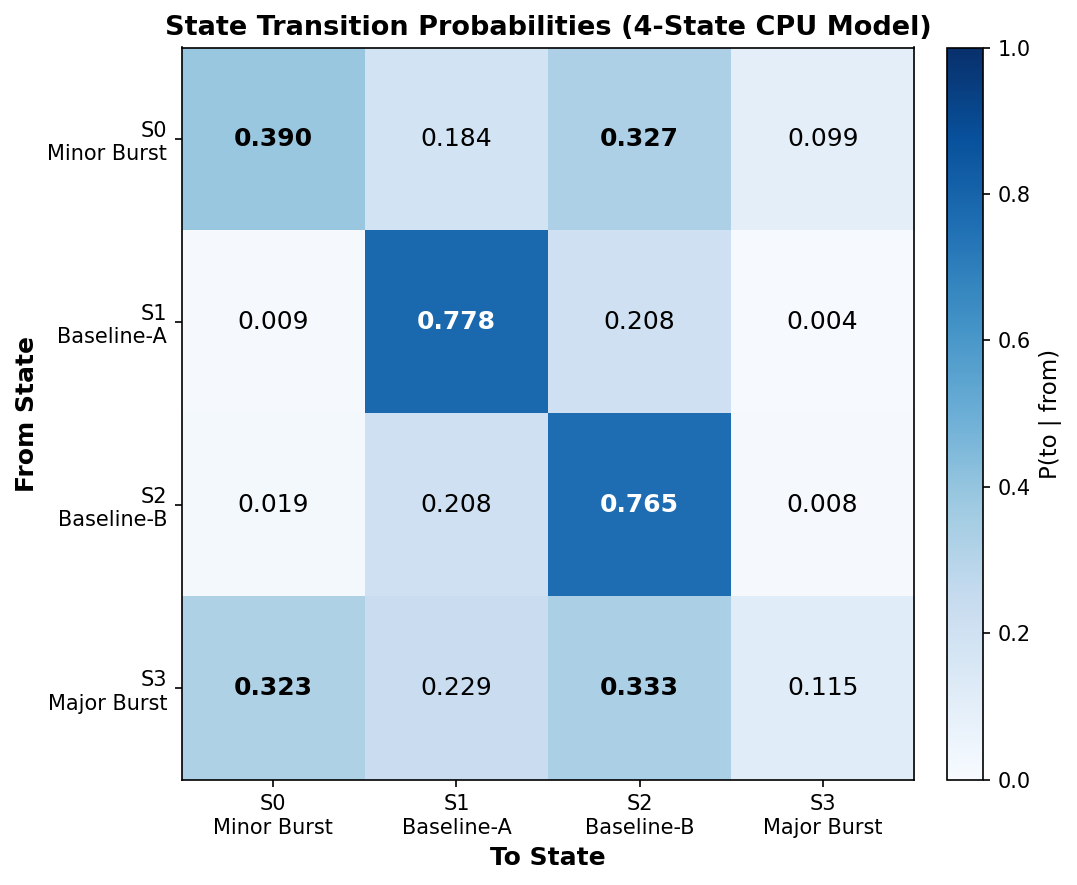
\includegraphics[width=0.6\textwidth]{figures/fig3_transition_matrix.png}
\caption{\textbf{State transition dynamics.} Within-day transition probability matrix for the 4-state CPU model. Baseline states (S1, S2) are highly self-sustaining (diagonal $\approx 0.77$) with symmetric exchange ($P \approx 0.208$). Burst states (S0, S3) are transient excursions that exit preferentially to baselines.}
\label{fig:transitions}
\end{figure}

\subsection{Developmental Trajectory}

The learned representations capture a developmental trajectory without any temporal labels (Table~\ref{tab:development}).

\begin{table}[h]
\centering
\caption{Developmental trajectory across 5 recording days (CPU, 4-state model).}
\label{tab:development}
\begin{tabular}{@{}lcccl@{}}
\toprule
Day & Duration & Dominant State & Entropy (bits) & Interpretation \\
\midrule
0 & $\sim$11\,h & S1 (89\%) & 0.511 & Initial mono-state \\
1 & $\sim$7\,h & S2 emerging (63\%) & 1.042 & Bistability onset \\
2 & $\sim$4\,h & S2 dominant (94\%) & 0.410 & State consolidation \\
3 & $\sim$4\,h & S2 (80\%) + bursts & 0.951 & Burst emergence \\
4 & $\sim$1\,h & All states active & 1.918 & Dynamic complexity peak \\
\bottomrule
\end{tabular}
\end{table}

State entropy increases from 0.511 bits (day 0) to 1.918 bits (day 4, near the theoretical maximum of 2.0 bits for 4 states). The trajectory is not monotonic---day 2 shows a transient entropy decrease during state consolidation---but the overall trend is clear: the organoid's dynamical repertoire expands over the recording period.

Burst states (S0, S3) are absent on day 0 and become prominent on day 4, where they account for 51\% of windows (Figure~\ref{fig:development}). This pattern is consistent with \textit{in vitro} neural network maturation: as synaptic connectivity increases, the network develops the capacity for coordinated high-activity events.

\begin{figure}[t]
\centering
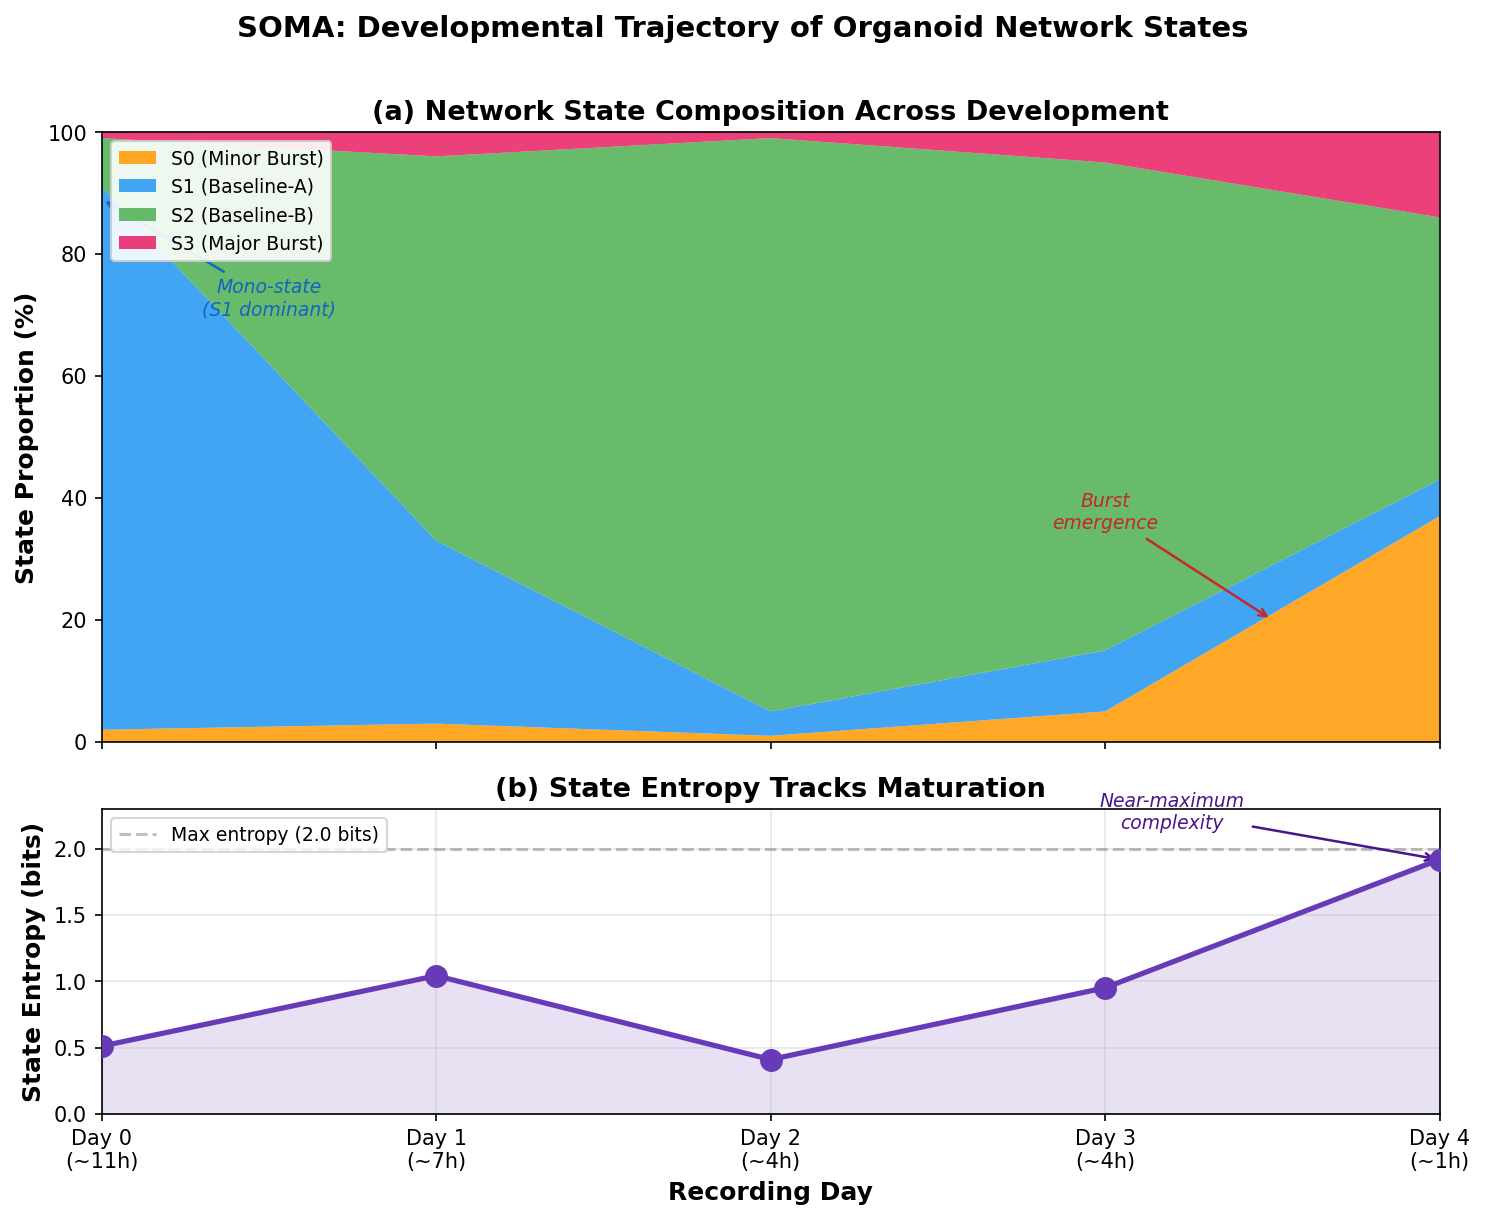
\includegraphics[width=\textwidth]{figures/fig4_developmental_trajectory.png}
\caption{\textbf{Developmental trajectory across 5 recording days.} Left: State proportion stacked area chart showing gradual shift from mono-state (day 0) to multi-state dynamics (day 4). Right: State entropy increases from 0.51 to 1.92 bits, reflecting expanding dynamical repertoire consistent with neural maturation.}
\label{fig:development}
\end{figure}

\subsection{Split-Half Validation}

Split-half reliability testing confirms that the discovered states are intrinsic to the organoid, not artifacts of a specific training run. Four independent models---two trained on CPU, two on GPU---all converge on the same binary state structure (Table~\ref{tab:splithalf}).

\begin{table}[h]
\centering
\caption{Split-half validation: independent models on non-overlapping data.}
\label{tab:splithalf}
\begin{tabular}{@{}lccccc@{}}
\toprule
& \multicolumn{2}{c}{CPU (20ep)} & \multicolumn{2}{c}{GPU (30ep)} \\
\cmidrule(lr){2-3} \cmidrule(lr){4-5}
Metric & Half A & Half B & Half A & Half B \\
\midrule
Windows & 2,509 & 2,538 & 8,898 & 9,014 \\
Optimal $k$ & 2 & 2 & 2 & 2 \\
Silhouette & 0.575 & 0.625 & 0.703 & 0.699 \\
Dominant state \% & 65.8 & 66.5 & 93.9 & 93.7 \\
\bottomrule
\end{tabular}
\end{table}

The GPU split-half achieves the strongest results: silhouette difference of 0.004, dominant state proportion difference of 0.2\%, and consistent state counts (8,359/539 vs.\ 8,449/565). This level of agreement across independent training runs on non-overlapping data provides strong evidence that the discovered states reflect genuine properties of the organoid's network dynamics (Figure~\ref{fig:splithalf_fig}).

\begin{figure}[t]
\centering
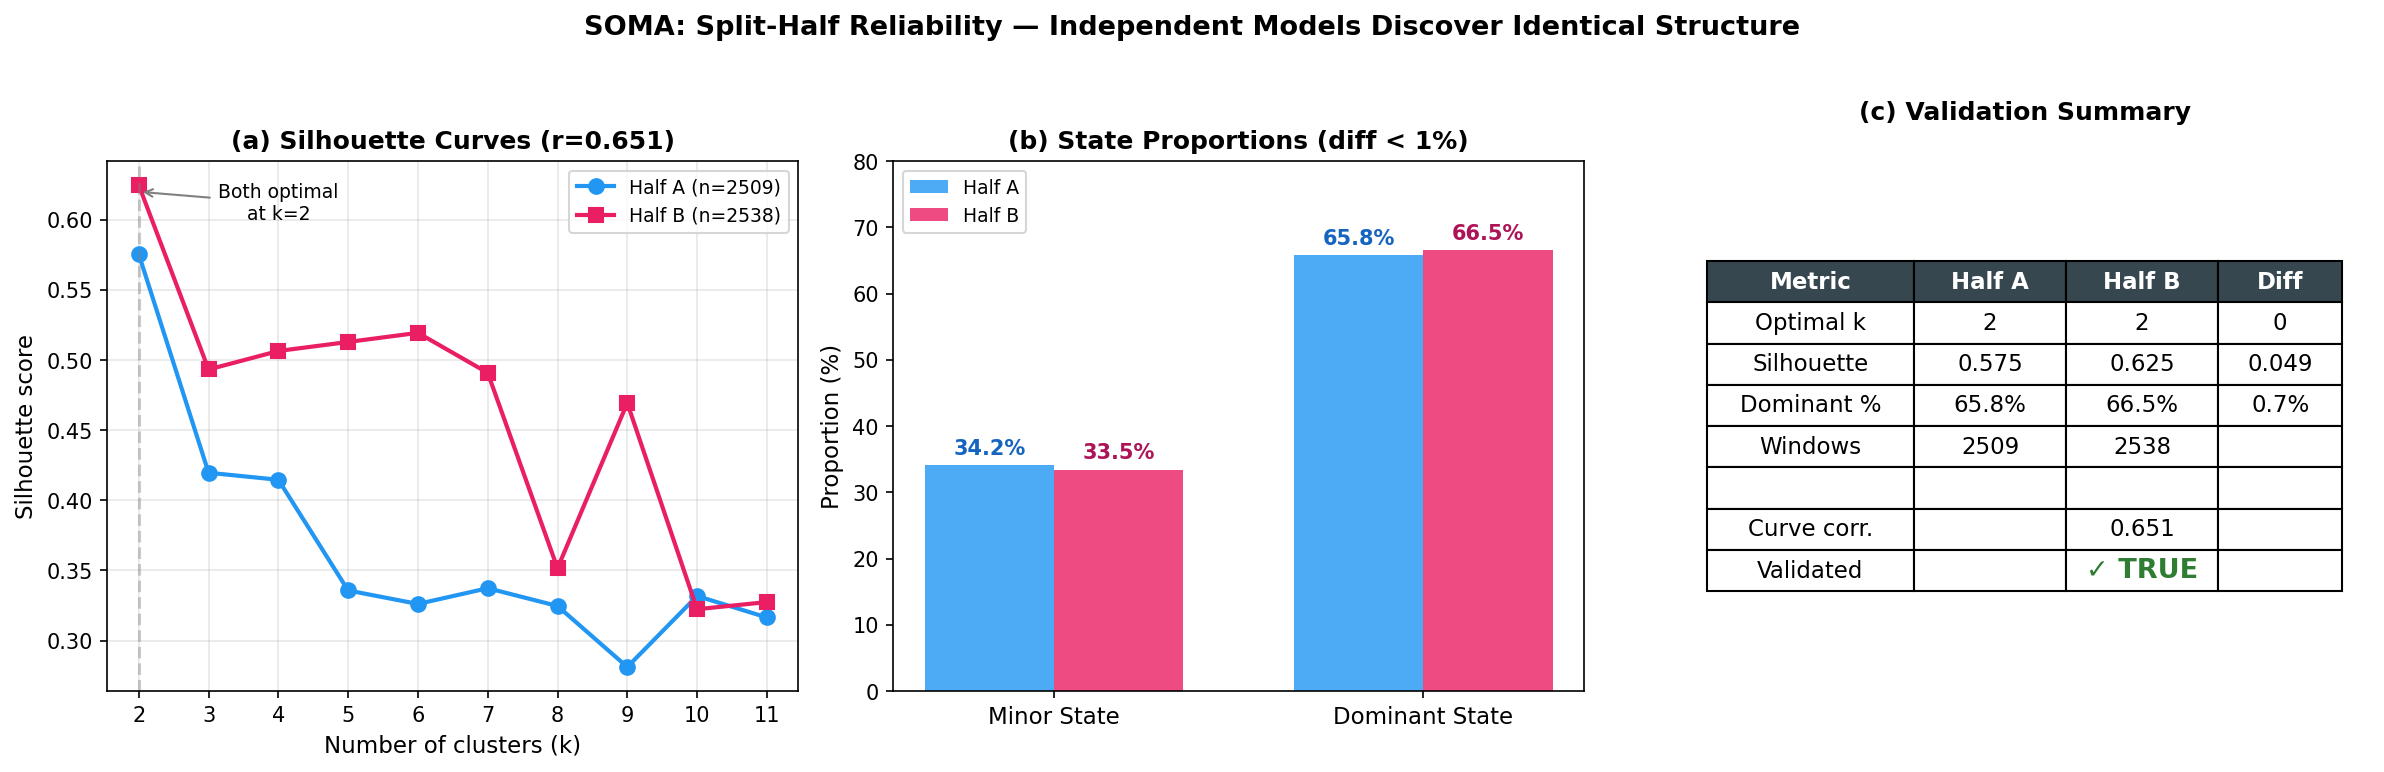
\includegraphics[width=\textwidth]{figures/fig5_split_half_validation.png}
\caption{\textbf{Split-half validation.} Independent SOMA models trained on interleaved non-overlapping data discover identical state structure. Left: Silhouette curves for Half A vs.\ Half B. Center: State proportion comparison. Right: Agreement metrics across CPU and GPU scales.}
\label{fig:splithalf_fig}
\end{figure}

\subsection{Auxiliary Validation}

\paragraph{Spike rate encoding.} Embedding norm correlates with mean spike rate at $r = -0.648$ (CPU) and $r = -0.245$ (GPU). The weaker GPU correlation reflects distributional encoding: with more dimensions available, spike-rate information is encoded across the representation rather than concentrated in the norm. Both correlations are significant ($p < 10^{-5}$).

\paragraph{Embedding geometry.} PCA of the 256-dim GPU embeddings captures 55.8\% variance in 2 components, with 15 components required for 95\%. The participation ratio of 9.47 indicates the effective embedding dimensionality matches the number of discovered states, suggesting the model uses its capacity efficiently.

% ============================================================
% 5. DISCUSSION
% ============================================================
\section{Discussion}

\paragraph{Biological interpretation.}
The 4-state structure discovered by SOMA maps to a biologically plausible model of organoid network dynamics. Two stable baseline configurations (S1 and S2) with distinct spatial patterns---one dominated by electrode 23, the other by electrode 15---suggest two competing network assemblies. Their symmetric switching ($P \approx 0.208$) resembles bistable dynamics observed in cortical cultures and models near the critical point between ordered and disordered phases.

The burst states (S0, S3) are transient perturbations that disrupt the baseline oscillation, consistent with population burst events reported in organoid electrophysiology \citep{trujillo2019complex}. Their emergence on later recording days aligns with the developmental expectation that increased synaptic connectivity enables coordinated network events.

\paragraph{Hierarchical structure.}
The $2 \rightarrow 4 \rightarrow 9$ state hierarchy across model scales is a key finding. Rather than discovering qualitatively different structures at different scales, the model reveals nested organization: the binary split into two baseline configurations is the most fundamental feature, burst modes appear as a second level, and fine-grained sub-states emerge with sufficient model capacity. This hierarchy is characteristic of real neural state spaces, where coarse dynamics (e.g., sleep vs.\ wake) encompass finer sub-states (e.g., NREM stages).

The absence of a silhouette plateau in the GPU model (silhouette increases monotonically through $k=9$) suggests additional structure may exist beyond what the current data can resolve. With denser MEAs and longer recordings, even finer state distinctions may emerge.

\paragraph{Methodological implications.}
SOMA requires no labeled data, no assumptions about what features matter, and minimal configuration (only patch size adapts to the electrode layout). This makes it a general-purpose tool for organoid electrophysiology: any MEA recording can be analyzed by the same pipeline. The architecture auto-configures for different electrode counts and temporal resolutions, as demonstrated by its successful application to both 32-channel organoid MEA (10 time bins) and 64-channel scalp EEG (160 time points) with only patch size adjustment.

\paragraph{Limitations.}
Several limitations should be noted. First, all results derive from a single organoid (fs437) from one recording session. Replication across organoids, labs, and MEA platforms is the critical next step for establishing generalizability. Second, there is no ground-truth labeling of organoid network states---our validation relies on split-half reliability and biological plausibility rather than comparison to a gold standard. Third, burst states are rare (3.8\% combined), so their characterization rests on relatively few observations. Fourth, day 4 data is the shortest segment ($\sim$1 hour, 401 windows for the CPU model); the entropy peak at day 4 should be interpreted cautiously. Finally, the EEG cross-substrate validation (meditation/rest paradigm) yielded a null result (silhouette $\approx 0$), suggesting that the current condition labeling (depth-threshold meditation) does not produce separable states in SOMA embeddings. Different experimental paradigms may be needed for EEG validation.

% ============================================================
% 6. CONCLUSION
% ============================================================
\section{Conclusion}

We have introduced SOMA, a self-supervised architecture that discovers discrete network states in brain organoid MEA recordings without labels, hand-crafted features, or prior assumptions. The discovered states are hierarchically organized, temporally structured, validated by split-half reliability, and track developmental maturation. This work demonstrates that modern self-supervised learning methods---originally developed for computer vision---can be productively adapted to the radically different domain of organoid electrophysiology.

SOMA provides a foundation for hypothesis-free analysis of organoid network dynamics. Future work includes: (1) validation across multiple organoids and MEA platforms, (2) analysis of stimulation-response dynamics in the learned state space, (3) real-time state monitoring during closed-loop experiments, and (4) extension to high-density MEA recordings with thousands of electrodes.

\paragraph{Acknowledgments.}
We thank the FinalSpark team---Fred Jordan, Martin Kutter, Jean-Marc Comby, Flora Brozzi, and Dr.\ Ewelina Kurtys---for developing the Neuroplatform and making brain organoid MEA recordings openly accessible. The organoid data used in this work (sample fs437) was recorded on the FinalSpark Neuroplatform. This work was conducted using an AI-assisted research workflow.

\paragraph{Data and code availability.}
The FinalSpark organoid data is available via the Neuroplatform \citep{jordan2024open}. Code and trained models will be released upon publication.

% ============================================================
% REFERENCES
% ============================================================
\bibliographystyle{plainnat}

\begin{thebibliography}{99}

\bibitem[Assran et~al.(2023)]{assran2023ijepa}
Assran, M., Duval, Q., Misra, I., Bojanowski, P., Vincent, P., Rabbat, M., LeCun, Y., and Ballas, N.
\newblock Self-supervised learning from images with a joint-embedding predictive architecture.
\newblock In \emph{Proceedings of CVPR}, 2023.

\bibitem[Bardes et~al.(2024)]{bardes2024vjepa}
Bardes, A., Garrido, Q., Ponce, J., Chen, X., Rabbat, M., LeCun, Y., Assran, M., and Ballas, N.
\newblock V-JEPA: Latent video prediction for visual representation learning.
\newblock \emph{arXiv preprint arXiv:2404.08471}, 2024.

\bibitem[Beggs and Plenz(2003)]{beggs2003neuronal}
Beggs, J.~M. and Plenz, D.
\newblock Neuronal avalanches in neocortical circuits.
\newblock \emph{Journal of Neuroscience}, 23(35):11167--11177, 2003.

\bibitem[Jordan et~al.(2024)]{jordan2024open}
Jordan, F., Kutter, M., Comby, J.-M., Brozzi, F., and Kurtys, E.
\newblock Open and remotely accessible Neuroplatform for research in wetware computing.
\newblock \emph{Frontiers in Artificial Intelligence}, 7:1376042, 2024.

\bibitem[Kostas et~al.(2021)]{kostas2021bendr}
Kostas, D., Aroca-Ouellette, S., and Rudzicz, F.
\newblock BENDR: Using transformers and a contrastive self-supervised learning task to classify EEG data.
\newblock \emph{Frontiers in Human Neuroscience}, 15:653659, 2021.

\bibitem[Lancaster et~al.(2013)]{lancaster2013cerebral}
Lancaster, M.~A., Renner, M., Martin, C.-A., Wenzel, D., Bicknell, L.~S., Hurles, M.~E., Homfray, T., Penninger, J.~M., Jackson, A.~P., and Knoblich, J.~A.
\newblock Cerebral organoids model human brain development and microcephaly.
\newblock \emph{Nature}, 501(7467):373--379, 2013.

\bibitem[Dong et~al.(2024)]{dong2024brainjepa}
Dong, Z., Li, R., Wu, Y., Nguyen, T.~T., Chong, J.~S.~X., Ji, F., Tong, N.~R.~J., Chen, C.~L.~H., and Zhou, J.~H.
\newblock Brain-JEPA: Brain dynamics foundation model with gradient positioning and spatiotemporal masking.
\newblock In \emph{Advances in Neural Information Processing Systems (NeurIPS)}, 2024. Spotlight.

\bibitem[Pa\c{s}ca(2019)]{pasca2019assembloids}
Pa\c{s}ca, S.~P.
\newblock Assembling human brain organoids.
\newblock \emph{Science}, 363(6423):126--127, 2019.

\bibitem[Rousseeuw(1987)]{rousseeuw1987silhouettes}
Rousseeuw, P.~J.
\newblock Silhouettes: A graphical aid to the interpretation and validation of cluster analysis.
\newblock \emph{Journal of Computational and Applied Mathematics}, 20:53--65, 1987.

\bibitem[Sharf et~al.(2022)]{sharf2022functional}
Sharf, T., van~der~Molen, T., Glasauer, S.~M.~K., Guzman, E., Buccino, A.~P., Luna, G., Cheng, Z., Audouard, M., Ranasinghe, K.~G., Kudo, K., Nagarajan, S.~S., Tovar, K.~R., Petzold, L.~R., Hierlemann, A., Hansma, P.~K., and Kosik, K.~S.
\newblock Functional neuronal circuitry and oscillatory dynamics in human brain organoids.
\newblock \emph{Nature Communications}, 13:4403, 2022.

\bibitem[Trujillo et~al.(2019)]{trujillo2019complex}
Trujillo, C.~A., Gao, R., Negraes, P.~D., Gu, J., Buchanan, J., Preissl, S., Wang, A., Wu, W., Haddad, G.~G., Chaim, I.~A., Domissy, A., Vandenberghe, M., Devor, A., Yeo, G.~W., Voytek, B., and Muotri, A.~R.
\newblock Complex oscillatory waves emerging from cortical organoids model early human brain network development.
\newblock \emph{Cell Stem Cell}, 25(4):558--569, 2019.

\bibitem[Cui et~al.(2024)]{cui2024neurogpt}
Cui, W., Jeong, W., Th\"{o}lke, P., Medani, T., Jerbi, K., Joshi, A.~A., and Leahy, R.~M.
\newblock NeuroGPT: Towards a foundation model for EEG.
\newblock \emph{arXiv preprint arXiv:2311.03764}, 2024.

\bibitem[Zbontar et~al.(2021)]{zbontar2021barlow}
Zbontar, J., Jing, L., Misra, I., LeCun, Y., and Deny, S.
\newblock Barlow Twins: Self-supervised learning via redundancy reduction.
\newblock In \emph{Proceedings of ICML}, 2021.

\end{thebibliography}

\end{document}

